\documentclass{article}
% General document formatting
    \usepackage[margin=1.3in]{geometry}
    \usepackage[parfill]{parskip}
    \usepackage[utf8]{inputenc}
     \usepackage{graphicx}   
    % Related to math
    \usepackage{amsmath,amssymb,amsfonts,amsthm}
    
    \usepackage[backend=biber]{biblatex}
    \addbibresource{prop.bib}

\title{Predicting phage-host relationships using network fusion}
\author{Hielke Walinga (4373561) \\ hielkewalinga@gmail}
\date{\today}

\begin{document}

\maketitle

\section{Introduction}

Here we propose a method for predicting the phage-host relationships 
by combining different metrics using network fusion techniques.

\subsection{Motivation}

Bacteria are under a constant barrage of phages that act as viruses and
integrate their DNA into the bacteria so that they can be multiplied. 
The bacterial communities are very diverse and almost all suffer from
attachs by phages. Next to that, there is a lot of information about
these attacks found in the DNA of both the phages and the bacteria. 
That makes this an interesting subject to learn more about ecological 
networks on the micro scale.

\subsection{Network fusion}

When creating a network from biological data, a common challenge involves
being able to combine multiple sources of information. This problem is
known as network fusion. 

There are multiple different strategies to solve the network fusion problem. 
Here we propose to make use of an existing method called 
similarity network fusion (SNF)~\cite{wang2014similarity}
with more details here~\cite{wang2012unsupervised}

For a full explenation of the algorithm,
consult the papers, but in short, you have to create a similarity network
for each source of information and then combine the networks using the 
following algorithm:

First generate a similarity matrix $W$ for each of your information sources, 
then normalize this matrix to create the status matrix.
Take the self-similarity as $\frac{1}{2}$.
Then create a kernel matrix $P$ 
by normalizing using the k-nearest neighbours $N_i$ which 
results in a sparse matrix $P^*$.

\begin{equation}
    P(i, j) = 
    \begin{cases}
        \cfrac{W(i, j)}{2 \sum_{k \neq i}W(i, k)} & j \neq i \\
        \hfil \frac{1}{2} & j = i
    \end{cases}
\end{equation}

\begin{equation}
    P^*(i, j) = 
    \begin{cases}
        \cfrac{W(i, j)}{\sum_{i \in N_j}W(i, j)} & i \in N_j \\
        \hfil 0 & else
    \end{cases}
\end{equation} 

Here are the update formulas to fuse the different status matrices $P_v$ and $P_w$ that 
represent two different information sources. Repeat the formulas till convergence.

\begin{align}
    \begin{split}
        P_{v, t+1} = P^*_{w, t} \times P_{v, t} \times P^{*,T}_{w, t} \\
        P_{w, t+1} = P^*_{v, t} \times P_{w, t} \times P^{*,T}_{v, t}
    \end{split}
\end{align}

This can be extended to account for more than 2 information sources.

\subsection{Representing the phage-host relationships in a bipartite graph}

A bipartite graph is a network in which the vertices can be divided into two 
groups in which there are only links from one group to the other. 

The phage-host relationships can be represented in a bipartite graph. 
Such a relationship is usually represented as a relation matrix in which 
an edge represents the possibility for a phage to be able to infect the 
bacteria.

\subsection{Modularity and nestedness}

\ldots

\begin{figure}[h]
\centering
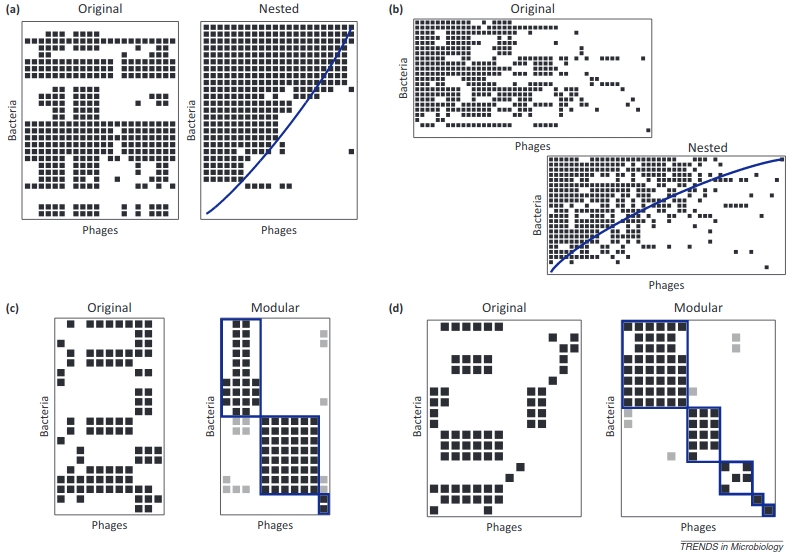
\includegraphics[width=0.5\textwidth]{img/nested-vs-modular.png}
\caption{Nestedness vs.\ modular infection matrices}
\end{figure}

\subsection{What data is available}

The proposed method tries to use information that is available for as well
phage-host relationships as well as phage-phage and bacterium-bacterium
relationships / similarities. Here summarized what these kinds of sources
of information are.

\subsubsection{Data sources for phage-host relationships}

\subsubsection{Data sources for phage-phage relationships}

\subsubsection{Data sources for bacterium-bacterium relationships}

\section{Related work}

As far as I can find, the only computational work done on phage-host relationships 
involves a single metric which is used to measure the possibility of a phage-host relationship~\cite{edwards2016computational}.
I could not find references to an attempt to combine this result or to combine
it with phage-phage or bacterium-bacterium similarity.

\section{Proposed method}

\subsection{Combining different information}

First, the different sources of information for both the phages as the bacteria networks
are combined to present a similarity graph for both the phages and the bacteria.
For this the standard SNF method can be used.

\subsection{Diffusion of the phage-host relationship}

Now we have a similarity network for both the phages as the bacteria. 
The next step will be to `diffuse' the information that exist for phage-host 
relationships (the connection graph) 
to other phage-host connection that don't have this information
available.  
We diffuse the weights to other connections that have the most similar phages
or the bacteria.

To do this we first pick what network to use (either the phage-phage $F$, or 
the bacterium-bacterium $B$). (It is probably best to make use of the sparse
similarity matrix here, $F^*$ and $B^*$.).
Then multiply this with the connection matrix. This will then move the
weights over the strongest connection for each phage or bacterium.
When working out the math it will become clear that this method can be done in a single 
step and has much resemblance to the previous discussed SNF algorithm. 

\begin{align}
    \begin{split}
    C_{t+1} &= F^* \times C_t \\
    C_{t} &= (B^* \times C_{t - 1}^{T})^{T} \\
          &= C_{t - 1} \times B^{*,T} \\
    \hfil Combined: \\
    C_{t+1} &= F^* \times C_{t - 1} \times B^{*,T}
    \end{split}
\end{align}

\subsubsection{Alteration to ensure convergence}

Since we are alternating between two different similarity matrices, I don't think it will
converge. To make sure the algorithm converges, I propose to alter the
similarity matrices every iteration by gradually reducing the percentage of weight
that gets moved around until it reaches zero percent.

This can be mathematically be accomplished by changing the normalization
function so the self-similarity start at some point ($a(0) = \frac{1}{2}$) and gradually 
grows to one in which case all similarity is the self-similarity 
(i.e.\ the similarly matrix is an identity matrix)
and no weight is shifted anymore.

\begin{equation}
    \begin{gathered}
    P^*(i, j) = 
    \begin{cases}
        (1 - a(t)) \times \cfrac{W(i, j)}{\sum_{i \in N_j}W(i, j)} & i \in N_j \\
        \hfil a(t) & i = j \\
        \hfil 0 & else
    \end{cases} \\
    a(0) = \frac{1}{2} \\
    a(T) = 1
    \end{gathered}
\end{equation}

Additionally, this adjustment can help to prevent weights drift to far away and
can thereby preserve some nestedness. It is probably also best
that this function that is responsible for reducing the amount of shifted weight
is convex so that most of the change happens in the 
first iteration. I believe this will be best to prevent disrupting the 
nestedness too much.

\subsubsection{Performing network fusion on the connection matrix}

Now we only are left with multiple connection matrices for each source of 
information on the phage-host relationships. We can however transform the
connection matrix in a square matrix ($M$) by adding the missing edges between
bacteria and phages as an edge with zero. So, in essence we stack
the connection matrix with the similarity matrix of the phages and the bacteria.
The resulting matrices can then
be fused using the aforementioned SNF fusion algorithm. This can in fact
be reduced to applying something similar to the SNF fusion algorithm to the connection matrix 
directly:

\begin{gather*}
    \textit{Full matrix from connection matrix:} \\
    M = \begin{bmatrix}
            0 & C^T \\
            C & 0
        \end{bmatrix} 
\end{gather*}
\begin{gather*}
    \textit{Update rules:} \\
    M_{v, t+1} = M^*_{w, t} \times M_{v, t} \times M^{*,T}_{w, t} \\
    M_{w, t+1} = M^*_{v, t} \times M_{w, t} \times M^{*,T}_{v, t}
\end{gather*}
\begin{align*}
    M_{v, t+1} &= M^*_{w, t} \times M_{v, t} \times M^{*,T}_{w, t} \\
               &= \begin{bmatrix}
                   0_b & C^{*,T}_w \\
                   C^*_w & 0_f
               \end{bmatrix} \times 
               \begin{bmatrix}
                   0_b & C^T_v \\
                   C_v & 0_f
               \end{bmatrix} \times
               \begin{bmatrix} 
                   0_b & C^{*,T}_w \\
                   C^*_w & 0_f
               \end{bmatrix} \\
               &= \begin{bmatrix}
                   0_b & C^{*,T}_w C_v C^{*,T} \\
                   C^*_w C^T_v C^*_w & 0_f
                   \end{bmatrix} \\
           C_v &= C^{*,T}_w C_v C^{*,T}
\end{align*}

\subsubsection{A note on the order and combination of steps}

As can be seen, there are a few different ways to combine all the information.
You can for example also apply the network fusion on the connection matrix
first and then diffuse it using the similarity matrices. This is also 
faster because then the diffusion is only applied to one connection matrix
and not multiple. I think this might be a worthwhile alternative to investigate.

On the other hand, you can even apply the diffusion
using the different sources of the similarity matrices. I, however, don't
think that is the best way as it then will start to mix different kinds 
of information too much too early.

Finally, you can
also create the square matrix from the connection matrix by including the
similarity weights already instead of setting those edges to zero. I also 
think that such an approach tries to combine too much information too early.
However, it might still be interesting to investigate the affect between
forcefully setting the similarities between bacteria and phages to zero 
or to let them grow as well, or even initialize them to some value (fixed
or otherwise).

\subsubsection{A note on computational complexity}

To reduce the computational I propose to make the similarity matrices sparse by only
looking at the k-nearest neighbours for each similarity neighbour.
This is also done in the SNF algorithm and can also trivially be applied 
to the aforementioned formulas.

\subsubsection{Notes on modular vs.\ nestedness}

The approach relies on the assumption that phage-host networks are
modular. I assume it would work best in situations where one wants to place
unknown bacteria or phages in a spot with already fairly known relationship. 

However, it should also work for relative nested networks, but only if it is 
true that generalized phages and general bacteria are relatively very 
similar to a lot of other resp.\ phages and 
the specialized phages / less targeted bacteria are more unique. 

\section{Summary}

The discussed method can be summarized in four steps (not necessarily in this order):

\begin{itemize}
\item Find similarity matrices for phage-phage and bacterium-bacterium using network fusion.
\item Find connection matrix for phage-host.
\item Diffuse the phage-host matrix using the phage-phage and bacterium-bacterium matrix.
\item Apply network fusion to the resulting diffused phage-host relationships.
 \end{itemize}

\section{Further ideas}

\subsection{Maximizing modularity}

Although modularity is not an end in itself, a good modular network is
something what we expect. That's why it might be worth looking into methods 
that focus on maximizing
the weights on the different information sources, 
instead of applying the network fusion algorithm.
This can be done on the connection matrix alone 
(and so still have the ability to perform network fusion and diffusion first),
but can also be done on the combined matrix with 
all the phage-phage and bacterium-bacterium information already included.  
This might however, force the modular network a bit too much.

\subsection{Using experimentally proven phage-host relationships}

There is various experimentally proven phage-host relationships available. 
These experimental data can be used to enhance the network fusion or 
to validate our method. 

Still, it is important to note that those experimentally reported phage-host
relationships might be biased and using it needs caution.

\subsubsection{Enhancing the proposal with some semi-supervised method}
It might be possible to use this as an alternative information source that
can make certain relationships more important than others because
of it being experimentally proven, or can be used in some semi-supervised
learning way.

\subsubsection{Validation}

This source of information can however also be used a way to validate
our method. 

It is perhaps also a good idea to see if certain assumptions we make in 
this proposal or true for the real world. 
Especially the idea that phages that infect the same
bacteria are more similar to each other and bacteria with the same phages
as viruses are more similar to each other.

\subsection{Deep learning approaches}

There might be a way to represent this problem in such a way that there is a 
way to work on this in a deep learning approach. Because of a lack of knowledge, 
I find it hard to come up with something related so far, but might still
be worth looking into.

\printbibliography{}

\end{document}
